% Created by tikzDevice version 0.12.3 on 2020-08-02 16:43:49
% !TEX encoding = UTF-8 Unicode
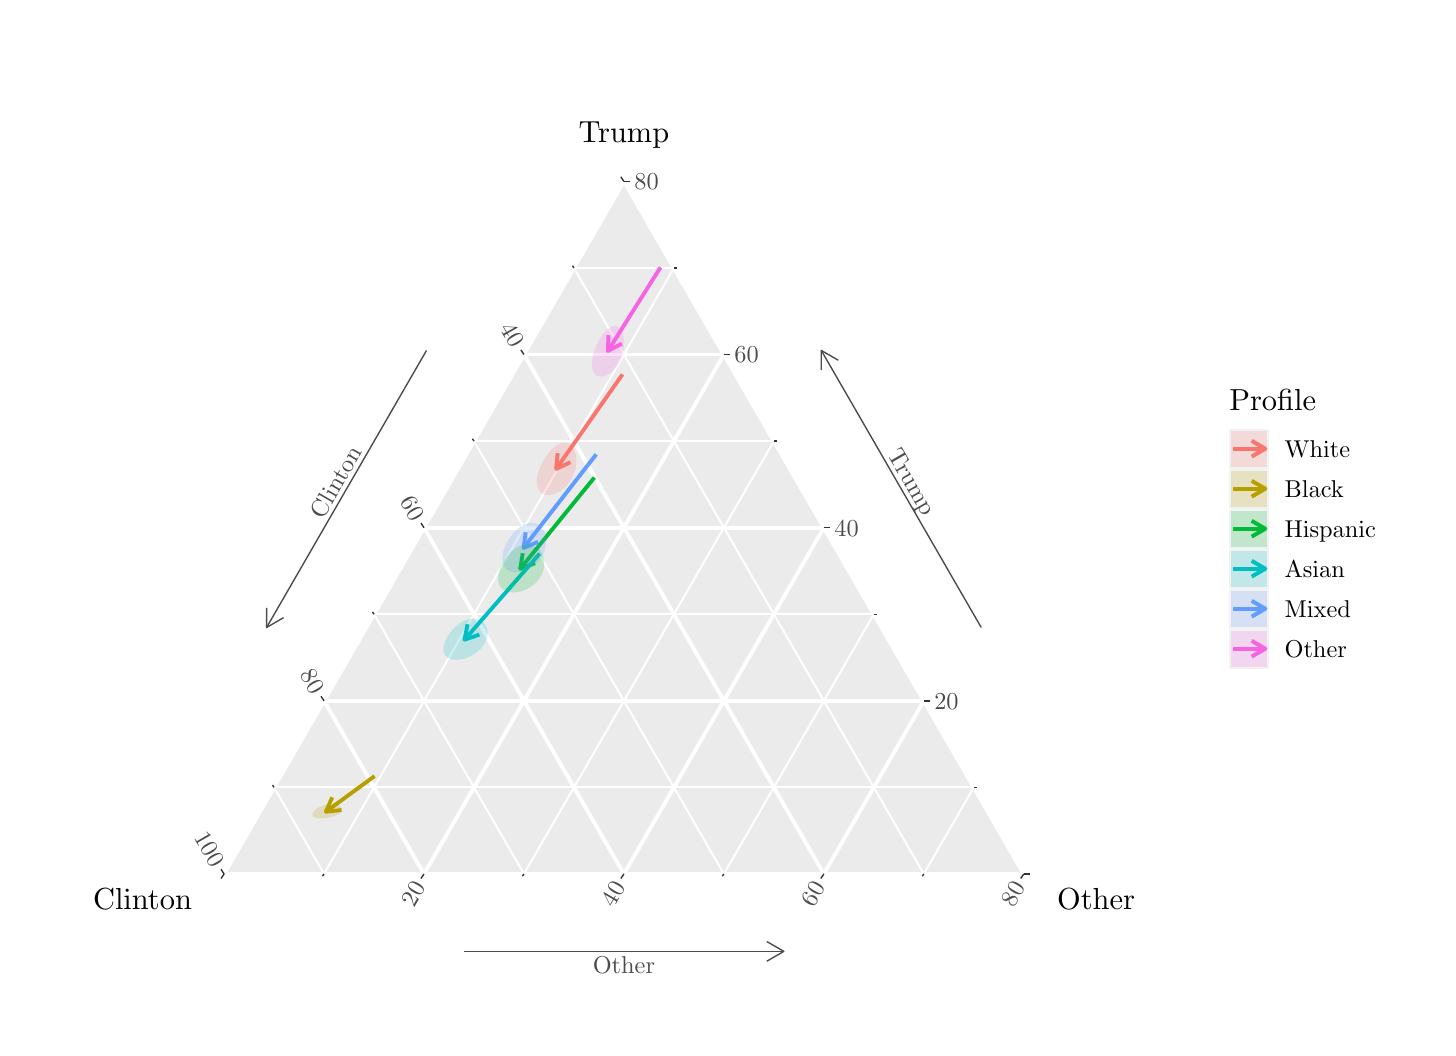
\begin{tikzpicture}[x=1pt,y=1pt]
\definecolor{fillColor}{RGB}{255,255,255}
\path[use as bounding box,fill=fillColor,fill opacity=0.00] (0,0) rectangle (505.89,361.35);
\begin{scope}
\path[clip] (  7.67,  0.00) rectangle (498.22,361.35);
\definecolor{drawColor}{RGB}{255,255,255}
\definecolor{fillColor}{RGB}{255,255,255}

\path[draw=drawColor,line width= 1.4pt,line join=round,line cap=round,fill=fillColor] (  7.67,  0.00) rectangle (498.22,361.35);
\end{scope}
\begin{scope}
\path[clip] ( 13.17,  5.50) rectangle (417.72,355.85);
\definecolor{fillColor}{gray}{0.92}

\path[fill=fillColor] (215.45,305.80) --
	( 70.97, 55.55) --
	(359.93, 55.55) --
	cycle;
\definecolor{drawColor}{RGB}{255,255,255}

\path[draw=drawColor,line width= 0.7pt,line join=round] (341.87, 86.83) -- ( 89.03, 86.83);

\path[draw=drawColor,line width= 0.7pt,line join=round] (305.75,149.39) -- (125.15,149.39);

\path[draw=drawColor,line width= 0.7pt,line join=round] (269.63,211.96) -- (161.27,211.96);

\path[draw=drawColor,line width= 0.7pt,line join=round] (233.51,274.52) -- (197.39,274.52);

\path[draw=drawColor,line width= 0.7pt,line join=round] (197.39,274.52) -- (323.81, 55.55);

\path[draw=drawColor,line width= 0.7pt,line join=round] (161.27,211.96) -- (251.57, 55.55);

\path[draw=drawColor,line width= 0.7pt,line join=round] (125.15,149.39) -- (179.33, 55.55);

\path[draw=drawColor,line width= 0.7pt,line join=round] ( 89.03, 86.83) -- (107.09, 55.55);

\path[draw=drawColor,line width= 0.7pt,line join=round] (107.09, 55.55) -- (233.51,274.52);

\path[draw=drawColor,line width= 0.7pt,line join=round] (179.33, 55.55) -- (269.63,211.96);

\path[draw=drawColor,line width= 0.7pt,line join=round] (251.57, 55.55) -- (305.75,149.39);

\path[draw=drawColor,line width= 0.7pt,line join=round] (323.81, 55.55) -- (341.87, 86.83);

\path[draw=drawColor,line width= 1.4pt,line join=round] (359.93, 55.55) -- ( 70.97, 55.55);

\path[draw=drawColor,line width= 1.4pt,line join=round] (323.81,118.11) -- (107.09,118.11);

\path[draw=drawColor,line width= 1.4pt,line join=round] (287.69,180.67) -- (143.21,180.67);

\path[draw=drawColor,line width= 1.4pt,line join=round] (251.57,243.24) -- (179.33,243.24);

\path[draw=drawColor,line width= 1.4pt,line join=round] (215.45,305.80) -- (215.45,305.80);

\path[draw=drawColor,line width= 1.4pt,line join=round] (215.45,305.80) -- (359.93, 55.55);

\path[draw=drawColor,line width= 1.4pt,line join=round] (179.33,243.24) -- (287.69, 55.55);

\path[draw=drawColor,line width= 1.4pt,line join=round] (143.21,180.67) -- (215.45, 55.55);

\path[draw=drawColor,line width= 1.4pt,line join=round] (107.09,118.11) -- (143.21, 55.55);

\path[draw=drawColor,line width= 1.4pt,line join=round] ( 70.97, 55.55) -- ( 70.97, 55.55);

\path[draw=drawColor,line width= 1.4pt,line join=round] ( 70.97, 55.55) -- (215.45,305.80);

\path[draw=drawColor,line width= 1.4pt,line join=round] (143.21, 55.55) -- (251.57,243.24);

\path[draw=drawColor,line width= 1.4pt,line join=round] (215.45, 55.55) -- (287.69,180.68);

\path[draw=drawColor,line width= 1.4pt,line join=round] (287.69, 55.55) -- (323.81,118.11);

\path[draw=drawColor,line width= 1.4pt,line join=round] (359.93, 55.55) -- (359.93, 55.55);
\definecolor{drawColor}{RGB}{245,100,227}

\path[draw=drawColor,line width= 1.4pt,line join=round] (228.68,274.75) -- (209.65,244.52);

\path[draw=drawColor,line width= 1.4pt,line join=round] (209.87,250.21) --
	(209.65,244.52) --
	(214.69,247.18);
\definecolor{drawColor}{RGB}{97,156,255}

\path[draw=drawColor,line width= 1.4pt,line join=round] (205.45,207.18) -- (179.19,173.39);

\path[draw=drawColor,line width= 1.4pt,line join=round] (179.97,179.03) --
	(179.19,173.39) --
	(184.46,175.54);
\definecolor{drawColor}{RGB}{248,118,109}

\path[draw=drawColor,line width= 1.4pt,line join=round] (214.94,236.07) -- (190.98,201.92);

\path[draw=drawColor,line width= 1.4pt,line join=round] (191.49,207.59) --
	(190.98,201.92) --
	(196.14,204.32);
\definecolor{drawColor}{RGB}{183,159,0}

\path[draw=drawColor,line width= 1.4pt,line join=round] (125.35, 90.90) -- (107.75, 78.03);

\path[draw=drawColor,line width= 1.4pt,line join=round] (110.05, 83.24) --
	(107.75, 78.03) --
	(113.41, 78.64);
\definecolor{drawColor}{RGB}{0,186,56}

\path[draw=drawColor,line width= 1.4pt,line join=round] (204.77,198.77) -- (177.99,165.82);

\path[draw=drawColor,line width= 1.4pt,line join=round] (178.89,171.44) --
	(177.99,165.82) --
	(183.31,167.85);
\definecolor{drawColor}{RGB}{0,191,196}

\path[draw=drawColor,line width= 1.4pt,line join=round] (185.01,171.31) -- (157.85,140.19);

\path[draw=drawColor,line width= 1.4pt,line join=round] (158.95,145.77) --
	(157.85,140.19) --
	(163.24,142.03);
\definecolor{fillColor}{RGB}{245,100,227}

\path[fill=fillColor,fill opacity=0.20] (215.41,248.99) --
	(215.46,248.47) --
	(215.49,247.94) --
	(215.50,247.39) --
	(215.48,246.83) --
	(215.45,246.26) --
	(215.39,245.68) --
	(215.31,245.10) --
	(215.20,244.51) --
	(215.07,243.93) --
	(214.92,243.35) --
	(214.75,242.77) --
	(214.55,242.20) --
	(214.33,241.64) --
	(214.09,241.09) --
	(213.83,240.56) --
	(213.55,240.05) --
	(213.26,239.55) --
	(212.94,239.07) --
	(212.61,238.61) --
	(212.27,238.18) --
	(211.91,237.78) --
	(211.54,237.40) --
	(211.16,237.04) --
	(210.78,236.72) --
	(210.38,236.43) --
	(209.99,236.17) --
	(209.59,235.94) --
	(209.19,235.74) --
	(208.79,235.58) --
	(208.40,235.46) --
	(208.01,235.36) --
	(207.63,235.30) --
	(207.26,235.28) --
	(206.91,235.29) --
	(206.56,235.34) --
	(206.23,235.42) --
	(205.92,235.54) --
	(205.62,235.69) --
	(205.35,235.87) --
	(205.09,236.09) --
	(204.86,236.34) --
	(204.65,236.62) --
	(204.47,236.93) --
	(204.30,237.27) --
	(204.17,237.64) --
	(204.05,238.03) --
	(203.97,238.45) --
	(203.91,238.89) --
	(203.87,239.35) --
	(203.86,239.84) --
	(203.88,240.34) --
	(203.92,240.86) --
	(203.98,241.40) --
	(204.07,241.94) --
	(204.18,242.50) --
	(204.31,243.06) --
	(204.47,243.63) --
	(204.64,244.21) --
	(204.84,244.78) --
	(205.05,245.36) --
	(205.28,245.93) --
	(205.52,246.50) --
	(205.78,247.06) --
	(206.06,247.61) --
	(206.34,248.14) --
	(206.64,248.66) --
	(206.95,249.17) --
	(207.26,249.65) --
	(207.58,250.12) --
	(207.91,250.56) --
	(208.25,250.98) --
	(208.58,251.37) --
	(208.92,251.73) --
	(209.26,252.06) --
	(209.61,252.37) --
	(209.95,252.63) --
	(210.29,252.87) --
	(210.62,253.07) --
	(210.95,253.23) --
	(211.28,253.36) --
	(211.60,253.45) --
	(211.92,253.50) --
	(212.23,253.52) --
	(212.52,253.50) --
	(212.81,253.43) --
	(213.09,253.34) --
	(213.36,253.20) --
	(213.62,253.03) --
	(213.86,252.82) --
	(214.09,252.57) --
	(214.30,252.29) --
	(214.50,251.98) --
	(214.69,251.64) --
	(214.85,251.26) --
	(215.00,250.86) --
	(215.13,250.43) --
	(215.24,249.97) --
	(215.34,249.49) --
	(215.41,248.99) --
	cycle;
\definecolor{fillColor}{RGB}{97,156,255}

\path[fill=fillColor,fill opacity=0.20] (187.06,178.24) --
	(187.19,177.74) --
	(187.29,177.22) --
	(187.35,176.68) --
	(187.39,176.14) --
	(187.40,175.58) --
	(187.37,175.02) --
	(187.31,174.45) --
	(187.21,173.88) --
	(187.08,173.31) --
	(186.92,172.74) --
	(186.73,172.18) --
	(186.51,171.63) --
	(186.25,171.08) --
	(185.96,170.55) --
	(185.64,170.02) --
	(185.30,169.52) --
	(184.93,169.03) --
	(184.53,168.56) --
	(184.11,168.11) --
	(183.66,167.68) --
	(183.20,167.28) --
	(182.72,166.90) --
	(182.22,166.55) --
	(181.71,166.22) --
	(181.19,165.92) --
	(180.66,165.65) --
	(180.13,165.41) --
	(179.59,165.20) --
	(179.05,165.03) --
	(178.52,164.88) --
	(177.99,164.76) --
	(177.46,164.68) --
	(176.95,164.63) --
	(176.44,164.61) --
	(175.96,164.63) --
	(175.49,164.67) --
	(175.03,164.75) --
	(174.60,164.87) --
	(174.19,165.01) --
	(173.81,165.19) --
	(173.45,165.39) --
	(173.12,165.63) --
	(172.81,165.90) --
	(172.54,166.19) --
	(172.30,166.51) --
	(172.08,166.86) --
	(171.90,167.24) --
	(171.76,167.64) --
	(171.64,168.06) --
	(171.56,168.51) --
	(171.51,168.97) --
	(171.49,169.46) --
	(171.51,169.96) --
	(171.55,170.48) --
	(171.63,171.01) --
	(171.74,171.55) --
	(171.88,172.10) --
	(172.05,172.66) --
	(172.24,173.22) --
	(172.47,173.78) --
	(172.71,174.35) --
	(172.99,174.91) --
	(173.28,175.47) --
	(173.60,176.03) --
	(173.94,176.57) --
	(174.30,177.10) --
	(174.67,177.62) --
	(175.06,178.13) --
	(175.47,178.61) --
	(175.89,179.08) --
	(176.32,179.52) --
	(176.76,179.94) --
	(177.21,180.33) --
	(177.67,180.69) --
	(178.13,181.02) --
	(178.60,181.32) --
	(179.07,181.59) --
	(179.54,181.82) --
	(180.01,182.02) --
	(180.48,182.18) --
	(180.95,182.30) --
	(181.41,182.38) --
	(181.86,182.43) --
	(182.30,182.44) --
	(182.74,182.40) --
	(183.17,182.33) --
	(183.58,182.22) --
	(183.98,182.07) --
	(184.36,181.89) --
	(184.73,181.66) --
	(185.08,181.40) --
	(185.41,181.11) --
	(185.72,180.79) --
	(186.00,180.43) --
	(186.27,180.04) --
	(186.50,179.63) --
	(186.72,179.19) --
	(186.90,178.73) --
	(187.06,178.24) --
	cycle;
\definecolor{fillColor}{RGB}{248,118,109}

\path[fill=fillColor,fill opacity=0.20] (198.10,206.94) --
	(198.18,206.41) --
	(198.24,205.86) --
	(198.27,205.30) --
	(198.27,204.72) --
	(198.25,204.13) --
	(198.19,203.53) --
	(198.11,202.93) --
	(198.00,202.32) --
	(197.85,201.72) --
	(197.68,201.12) --
	(197.48,200.52) --
	(197.26,199.93) --
	(197.00,199.35) --
	(196.72,198.78) --
	(196.42,198.23) --
	(196.09,197.69) --
	(195.73,197.17) --
	(195.36,196.67) --
	(194.96,196.19) --
	(194.55,195.73) --
	(194.12,195.30) --
	(193.67,194.90) --
	(193.22,194.52) --
	(192.75,194.18) --
	(192.27,193.86) --
	(191.79,193.58) --
	(191.31,193.32) --
	(190.82,193.10) --
	(190.34,192.92) --
	(189.85,192.76) --
	(189.38,192.65) --
	(188.91,192.56) --
	(188.45,192.52) --
	(188.01,192.50) --
	(187.58,192.53) --
	(187.17,192.59) --
	(186.78,192.68) --
	(186.40,192.81) --
	(186.05,192.97) --
	(185.73,193.17) --
	(185.42,193.39) --
	(185.15,193.66) --
	(184.90,193.95) --
	(184.68,194.27) --
	(184.49,194.63) --
	(184.33,195.01) --
	(184.20,195.42) --
	(184.09,195.86) --
	(184.02,196.32) --
	(183.98,196.80) --
	(183.97,197.30) --
	(183.99,197.82) --
	(184.04,198.36) --
	(184.12,198.92) --
	(184.22,199.48) --
	(184.36,200.06) --
	(184.52,200.65) --
	(184.70,201.24) --
	(184.91,201.84) --
	(185.15,202.44) --
	(185.40,203.04) --
	(185.68,203.63) --
	(185.98,204.22) --
	(186.29,204.81) --
	(186.62,205.38) --
	(186.97,205.93) --
	(187.33,206.48) --
	(187.70,207.00) --
	(188.09,207.51) --
	(188.48,207.99) --
	(188.88,208.45) --
	(189.29,208.88) --
	(189.71,209.28) --
	(190.12,209.66) --
	(190.54,210.00) --
	(190.97,210.30) --
	(191.39,210.58) --
	(191.81,210.81) --
	(192.23,211.01) --
	(192.64,211.17) --
	(193.05,211.29) --
	(193.45,211.37) --
	(193.84,211.41) --
	(194.23,211.41) --
	(194.60,211.37) --
	(194.96,211.29) --
	(195.31,211.17) --
	(195.65,211.00) --
	(195.97,210.80) --
	(196.27,210.57) --
	(196.56,210.29) --
	(196.83,209.98) --
	(197.07,209.63) --
	(197.30,209.26) --
	(197.51,208.85) --
	(197.69,208.41) --
	(197.85,207.95) --
	(197.99,207.46) --
	(198.10,206.94) --
	cycle;
\definecolor{fillColor}{RGB}{183,159,0}

\path[fill=fillColor,fill opacity=0.20] (112.90, 79.90) --
	(113.05, 79.77) --
	(113.18, 79.63) --
	(113.29, 79.49) --
	(113.37, 79.34) --
	(113.44, 79.19) --
	(113.48, 79.04) --
	(113.49, 78.88) --
	(113.48, 78.72) --
	(113.45, 78.56) --
	(113.39, 78.40) --
	(113.31, 78.24) --
	(113.20, 78.07) --
	(113.07, 77.91) --
	(112.92, 77.75) --
	(112.74, 77.60) --
	(112.55, 77.44) --
	(112.33, 77.29) --
	(112.09, 77.14) --
	(111.84, 77.00) --
	(111.57, 76.86) --
	(111.28, 76.73) --
	(110.98, 76.60) --
	(110.67, 76.48) --
	(110.35, 76.37) --
	(110.02, 76.26) --
	(109.68, 76.16) --
	(109.34, 76.07) --
	(108.99, 75.99) --
	(108.64, 75.91) --
	(108.29, 75.84) --
	(107.94, 75.78) --
	(107.59, 75.73) --
	(107.24, 75.69) --
	(106.90, 75.66) --
	(106.57, 75.63) --
	(106.25, 75.62) --
	(105.93, 75.61) --
	(105.63, 75.61) --
	(105.34, 75.62) --
	(105.06, 75.64) --
	(104.80, 75.67) --
	(104.55, 75.71) --
	(104.31, 75.75) --
	(104.09, 75.81) --
	(103.89, 75.87) --
	(103.70, 75.95) --
	(103.54, 76.03) --
	(103.39, 76.12) --
	(103.26, 76.21) --
	(103.14, 76.32) --
	(103.05, 76.43) --
	(102.98, 76.54) --
	(102.92, 76.67) --
	(102.88, 76.80) --
	(102.87, 76.93) --
	(102.87, 77.08) --
	(102.89, 77.22) --
	(102.93, 77.37) --
	(102.99, 77.53) --
	(103.06, 77.68) --
	(103.15, 77.84) --
	(103.27, 78.01) --
	(103.39, 78.17) --
	(103.54, 78.33) --
	(103.70, 78.50) --
	(103.87, 78.66) --
	(104.06, 78.82) --
	(104.27, 78.98) --
	(104.49, 79.14) --
	(104.72, 79.29) --
	(104.97, 79.44) --
	(105.22, 79.58) --
	(105.49, 79.72) --
	(105.77, 79.85) --
	(106.05, 79.97) --
	(106.35, 80.09) --
	(106.65, 80.20) --
	(106.96, 80.30) --
	(107.28, 80.39) --
	(107.59, 80.47) --
	(107.92, 80.54) --
	(108.24, 80.60) --
	(108.57, 80.65) --
	(108.89, 80.68) --
	(109.22, 80.71) --
	(109.54, 80.72) --
	(109.86, 80.72) --
	(110.17, 80.71) --
	(110.48, 80.69) --
	(110.78, 80.66) --
	(111.07, 80.62) --
	(111.34, 80.56) --
	(111.61, 80.49) --
	(111.87, 80.42) --
	(112.11, 80.33) --
	(112.33, 80.23) --
	(112.54, 80.13) --
	(112.73, 80.02) --
	(112.90, 79.90) --
	cycle;
\definecolor{fillColor}{RGB}{0,186,56}

\path[fill=fillColor,fill opacity=0.20] (186.17,170.45) --
	(186.33,169.95) --
	(186.45,169.44) --
	(186.54,168.92) --
	(186.60,168.38) --
	(186.63,167.84) --
	(186.62,167.29) --
	(186.58,166.73) --
	(186.50,166.18) --
	(186.39,165.62) --
	(186.24,165.07) --
	(186.05,164.53) --
	(185.84,163.99) --
	(185.59,163.46) --
	(185.30,162.94) --
	(184.99,162.44) --
	(184.64,161.95) --
	(184.26,161.48) --
	(183.86,161.03) --
	(183.43,160.60) --
	(182.98,160.19) --
	(182.50,159.80) --
	(182.01,159.44) --
	(181.49,159.10) --
	(180.97,158.79) --
	(180.43,158.51) --
	(179.88,158.26) --
	(179.32,158.03) --
	(178.76,157.83) --
	(178.19,157.67) --
	(177.63,157.53) --
	(177.07,157.43) --
	(176.52,157.35) --
	(175.98,157.31) --
	(175.44,157.30) --
	(174.92,157.32) --
	(174.42,157.38) --
	(173.94,157.46) --
	(173.47,157.58) --
	(173.03,157.72) --
	(172.62,157.90) --
	(172.23,158.10) --
	(171.86,158.34) --
	(171.53,158.60) --
	(171.22,158.89) --
	(170.95,159.21) --
	(170.71,159.55) --
	(170.50,159.92) --
	(170.33,160.31) --
	(170.19,160.73) --
	(170.08,161.16) --
	(170.00,161.62) --
	(169.96,162.09) --
	(169.96,162.58) --
	(169.98,163.08) --
	(170.04,163.60) --
	(170.14,164.13) --
	(170.26,164.66) --
	(170.41,165.21) --
	(170.60,165.75) --
	(170.81,166.30) --
	(171.05,166.85) --
	(171.31,167.40) --
	(171.60,167.94) --
	(171.92,168.48) --
	(172.25,169.01) --
	(172.61,169.53) --
	(172.99,170.03) --
	(173.39,170.52) --
	(173.80,170.99) --
	(174.23,171.44) --
	(174.67,171.87) --
	(175.12,172.27) --
	(175.59,172.65) --
	(176.06,173.00) --
	(176.54,173.32) --
	(177.03,173.60) --
	(177.52,173.86) --
	(178.01,174.08) --
	(178.50,174.27) --
	(179.00,174.42) --
	(179.49,174.53) --
	(179.98,174.60) --
	(180.46,174.64) --
	(180.93,174.64) --
	(181.40,174.60) --
	(181.86,174.52) --
	(182.30,174.41) --
	(182.73,174.26) --
	(183.15,174.07) --
	(183.55,173.84) --
	(183.93,173.58) --
	(184.30,173.29) --
	(184.64,172.97) --
	(184.96,172.61) --
	(185.25,172.23) --
	(185.52,171.82) --
	(185.77,171.38) --
	(185.98,170.93) --
	(186.17,170.45) --
	cycle;
\definecolor{fillColor}{RGB}{0,191,196}

\path[fill=fillColor,fill opacity=0.20] (165.76,144.70) --
	(165.90,144.29) --
	(166.01,143.87) --
	(166.10,143.43) --
	(166.14,142.98) --
	(166.16,142.52) --
	(166.14,142.05) --
	(166.09,141.58) --
	(166.01,141.10) --
	(165.89,140.63) --
	(165.74,140.15) --
	(165.55,139.68) --
	(165.33,139.21) --
	(165.08,138.74) --
	(164.80,138.29) --
	(164.49,137.85) --
	(164.15,137.41) --
	(163.78,136.99) --
	(163.39,136.59) --
	(162.98,136.20) --
	(162.54,135.82) --
	(162.08,135.47) --
	(161.60,135.13) --
	(161.11,134.82) --
	(160.60,134.53) --
	(160.09,134.25) --
	(159.56,134.01) --
	(159.03,133.78) --
	(158.50,133.58) --
	(157.97,133.41) --
	(157.43,133.26) --
	(156.91,133.14) --
	(156.38,133.04) --
	(155.87,132.97) --
	(155.37,132.93) --
	(154.88,132.91) --
	(154.41,132.92) --
	(153.96,132.96) --
	(153.53,133.02) --
	(153.11,133.12) --
	(152.72,133.23) --
	(152.36,133.38) --
	(152.02,133.55) --
	(151.71,133.74) --
	(151.43,133.96) --
	(151.17,134.21) --
	(150.95,134.47) --
	(150.76,134.76) --
	(150.60,135.08) --
	(150.47,135.41) --
	(150.37,135.76) --
	(150.30,136.13) --
	(150.26,136.52) --
	(150.26,136.92) --
	(150.29,137.34) --
	(150.34,137.77) --
	(150.43,138.22) --
	(150.55,138.67) --
	(150.69,139.13) --
	(150.87,139.60) --
	(151.07,140.08) --
	(151.30,140.55) --
	(151.55,141.03) --
	(151.82,141.50) --
	(152.12,141.98) --
	(152.44,142.44) --
	(152.79,142.91) --
	(153.15,143.36) --
	(153.52,143.80) --
	(153.92,144.22) --
	(154.33,144.64) --
	(154.75,145.03) --
	(155.18,145.41) --
	(155.63,145.76) --
	(156.08,146.09) --
	(156.54,146.40) --
	(157.01,146.68) --
	(157.48,146.94) --
	(157.95,147.16) --
	(158.43,147.36) --
	(158.90,147.53) --
	(159.38,147.66) --
	(159.85,147.76) --
	(160.31,147.83) --
	(160.77,147.87) --
	(161.22,147.87) --
	(161.65,147.84) --
	(162.08,147.78) --
	(162.50,147.68) --
	(162.90,147.56) --
	(163.28,147.39) --
	(163.65,147.20) --
	(163.99,146.98) --
	(164.32,146.73) --
	(164.62,146.45) --
	(164.90,146.15) --
	(165.16,145.82) --
	(165.39,145.47) --
	(165.59,145.10) --
	(165.76,144.70) --
	cycle;
\definecolor{fillColor}{RGB}{255,255,255}

\path[fill=fillColor] ( 13.17,  5.50) --
	( 13.17,355.85) --
	(215.45,355.85) --
	(215.45,305.80) --
	( 70.97, 55.55) --
	(359.93, 55.55) --
	(215.45,305.80) --
	(215.45,355.85) --
	(417.72,355.85) --
	(417.72,  5.50) --
	( 13.17,  5.50) --
	cycle;
\end{scope}
\begin{scope}
\path[clip] ( 13.17,  5.50) rectangle (417.72,355.85);

\path[] ( 13.17,  5.50) --
	( 13.17,355.85) --
	(417.72,355.85) --
	(417.72,  5.50) --
	( 13.17,  5.50) --
	( 13.17,  5.50);
\end{scope}
\begin{scope}
\path[clip] ( 13.17,  5.50) rectangle (417.72,355.85);
\definecolor{drawColor}{gray}{0.20}

\path[draw=drawColor,line width= 0.5pt,line join=round] (359.93, 55.55) -- (362.13, 55.55);

\path[draw=drawColor,line width= 0.5pt,line join=round] (323.81,118.11) -- (326.01,118.11);

\path[draw=drawColor,line width= 0.5pt,line join=round] (287.69,180.67) -- (289.89,180.67);

\path[draw=drawColor,line width= 0.5pt,line join=round] (251.57,243.24) -- (253.77,243.24);

\path[draw=drawColor,line width= 0.5pt,line join=round] (215.45,305.80) -- (217.65,305.80);

\path[draw=drawColor,line width= 0.5pt,line join=round] (341.87, 86.83) -- (342.97, 86.83);

\path[draw=drawColor,line width= 0.5pt,line join=round] (305.75,149.39) -- (306.85,149.39);

\path[draw=drawColor,line width= 0.5pt,line join=round] (269.63,211.96) -- (270.73,211.96);

\path[draw=drawColor,line width= 0.5pt,line join=round] (233.51,274.52) -- (234.61,274.52);

\path[draw=drawColor,line width= 0.5pt,line join=round] (215.45,305.80) -- (214.35,307.45);

\path[draw=drawColor,line width= 0.5pt,line join=round] (179.33,243.24) -- (178.23,244.89);

\path[draw=drawColor,line width= 0.5pt,line join=round] (143.21,180.67) -- (142.11,182.32);

\path[draw=drawColor,line width= 0.5pt,line join=round] (107.09,118.11) -- (105.99,119.76);

\path[draw=drawColor,line width= 0.5pt,line join=round] ( 70.97, 55.55) -- ( 69.87, 57.20);

\path[draw=drawColor,line width= 0.5pt,line join=round] (197.39,274.52) -- (196.84,275.34);

\path[draw=drawColor,line width= 0.5pt,line join=round] (161.27,211.96) -- (160.72,212.78);

\path[draw=drawColor,line width= 0.5pt,line join=round] (125.15,149.39) -- (124.60,150.22);

\path[draw=drawColor,line width= 0.5pt,line join=round] ( 89.03, 86.83) -- ( 88.48, 87.66);

\path[draw=drawColor,line width= 0.5pt,line join=round] ( 70.97, 55.55) -- ( 69.87, 53.90);

\path[draw=drawColor,line width= 0.5pt,line join=round] (143.21, 55.55) -- (142.11, 53.90);

\path[draw=drawColor,line width= 0.5pt,line join=round] (215.45, 55.55) -- (214.35, 53.90);

\path[draw=drawColor,line width= 0.5pt,line join=round] (287.69, 55.55) -- (286.59, 53.90);

\path[draw=drawColor,line width= 0.5pt,line join=round] (359.93, 55.55) -- (358.83, 53.90);

\path[draw=drawColor,line width= 0.5pt,line join=round] (107.09, 55.55) -- (106.54, 54.73);

\path[draw=drawColor,line width= 0.5pt,line join=round] (179.33, 55.55) -- (178.78, 54.73);

\path[draw=drawColor,line width= 0.5pt,line join=round] (251.57, 55.55) -- (251.02, 54.73);

\path[draw=drawColor,line width= 0.5pt,line join=round] (323.81, 55.55) -- (323.26, 54.73);
\definecolor{drawColor}{gray}{0.30}

\node[text=drawColor,anchor=base west,inner sep=0pt, outer sep=0pt, scale=  0.88] at (327.61,115.08) {20};

\node[text=drawColor,anchor=base west,inner sep=0pt, outer sep=0pt, scale=  0.88] at (291.49,177.64) {40};

\node[text=drawColor,anchor=base west,inner sep=0pt, outer sep=0pt, scale=  0.88] at (255.37,240.21) {60};

\node[text=drawColor,anchor=base west,inner sep=0pt, outer sep=0pt, scale=  0.88] at (219.25,302.77) {80};

\node[text=drawColor,rotate=-60.00,anchor=base east,inner sep=0pt, outer sep=0pt, scale=  0.88] at (174.80,245.05) {40};

\node[text=drawColor,rotate=-60.00,anchor=base east,inner sep=0pt, outer sep=0pt, scale=  0.88] at (138.68,182.49) {60};

\node[text=drawColor,rotate=-60.00,anchor=base east,inner sep=0pt, outer sep=0pt, scale=  0.88] at (102.56,119.93) {80};

\node[text=drawColor,rotate=-60.00,anchor=base east,inner sep=0pt, outer sep=0pt, scale=  0.88] at ( 66.44, 57.36) {100};

\node[text=drawColor,rotate= 60.00,anchor=base east,inner sep=0pt, outer sep=0pt, scale=  0.88] at (143.93, 50.71) {20};

\node[text=drawColor,rotate= 60.00,anchor=base east,inner sep=0pt, outer sep=0pt, scale=  0.88] at (216.17, 50.71) {40};

\node[text=drawColor,rotate= 60.00,anchor=base east,inner sep=0pt, outer sep=0pt, scale=  0.88] at (288.41, 50.71) {60};

\node[text=drawColor,rotate= 60.00,anchor=base east,inner sep=0pt, outer sep=0pt, scale=  0.88] at (360.65, 50.71) {80};

\path[draw=drawColor,line width= 0.5pt,line join=round] (344.56,144.61) -- (286.77,244.71);

\path[draw=drawColor,line width= 0.5pt,line join=round] (292.93,241.16) --
	(286.77,244.71) --
	(286.77,237.60);

\path[draw=drawColor,line width= 0.5pt,line join=round] (144.12,244.71) -- ( 86.33,144.61);

\path[draw=drawColor,line width= 0.5pt,line join=round] ( 86.33,151.73) --
	( 86.33,144.61) --
	( 92.49,148.17);

\path[draw=drawColor,line width= 0.5pt,line join=round] (157.65, 27.57) -- (273.24, 27.57);

\path[draw=drawColor,line width= 0.5pt,line join=round] (267.08, 24.01) --
	(273.24, 27.57) --
	(267.08, 31.13);

\node[text=drawColor,rotate=-60.00,anchor=base,inner sep=0pt, outer sep=0pt, scale=  0.88] at (317.05,195.63) {Trump};

\node[text=drawColor,rotate= 60.00,anchor=base,inner sep=0pt, outer sep=0pt, scale=  0.88] at (113.84,195.63) {Clinton};

\node[text=drawColor,anchor=base,inner sep=0pt, outer sep=0pt, scale=  0.88] at (215.45, 19.57) {Other};
\definecolor{drawColor}{RGB}{0,0,0}

\node[text=drawColor,anchor=base,inner sep=0pt, outer sep=0pt, scale=  1.10] at (215.45,319.79) {Trump};

\node[text=drawColor,anchor=base east,inner sep=0pt, outer sep=0pt, scale=  1.10] at ( 59.37, 42.87) {Clinton};

\node[text=drawColor,anchor=base west,inner sep=0pt, outer sep=0pt, scale=  1.10] at (372.03, 42.87) {Other};
\end{scope}
\begin{scope}
\path[clip] (  0.00,  0.00) rectangle (505.89,361.35);
\definecolor{fillColor}{RGB}{255,255,255}

\path[fill=fillColor] (428.72,124.21) rectangle (492.72,237.14);
\end{scope}
\begin{scope}
\path[clip] (  0.00,  0.00) rectangle (505.89,361.35);
\definecolor{drawColor}{RGB}{0,0,0}

\node[text=drawColor,anchor=base west,inner sep=0pt, outer sep=0pt, scale=  1.10] at (434.22,223.00) {Profile};
\end{scope}
\begin{scope}
\path[clip] (  0.00,  0.00) rectangle (505.89,361.35);
\definecolor{fillColor}{gray}{0.95}

\path[fill=fillColor] (434.22,201.98) rectangle (448.68,216.43);
\end{scope}
\begin{scope}
\path[clip] (  0.00,  0.00) rectangle (505.89,361.35);
\definecolor{drawColor}{RGB}{248,118,109}

\path[draw=drawColor,line width= 1.4pt,line join=round] (435.67,209.20) -- (447.23,209.20);

\path[draw=drawColor,line width= 1.4pt,line join=round] (442.30,206.36) --
	(447.23,209.20) --
	(442.30,212.05);
\end{scope}
\begin{scope}
\path[clip] (  0.00,  0.00) rectangle (505.89,361.35);
\definecolor{fillColor}{RGB}{248,118,109}

\path[fill=fillColor,fill opacity=0.20] (434.93,202.69) rectangle (447.96,215.72);
\end{scope}
\begin{scope}
\path[clip] (  0.00,  0.00) rectangle (505.89,361.35);
\definecolor{fillColor}{gray}{0.95}

\path[fill=fillColor] (434.22,187.52) rectangle (448.68,201.98);
\end{scope}
\begin{scope}
\path[clip] (  0.00,  0.00) rectangle (505.89,361.35);
\definecolor{drawColor}{RGB}{183,159,0}

\path[draw=drawColor,line width= 1.4pt,line join=round] (435.67,194.75) -- (447.23,194.75);

\path[draw=drawColor,line width= 1.4pt,line join=round] (442.30,191.90) --
	(447.23,194.75) --
	(442.30,197.59);
\end{scope}
\begin{scope}
\path[clip] (  0.00,  0.00) rectangle (505.89,361.35);
\definecolor{fillColor}{RGB}{183,159,0}

\path[fill=fillColor,fill opacity=0.20] (434.93,188.23) rectangle (447.96,201.26);
\end{scope}
\begin{scope}
\path[clip] (  0.00,  0.00) rectangle (505.89,361.35);
\definecolor{fillColor}{gray}{0.95}

\path[fill=fillColor] (434.22,173.07) rectangle (448.68,187.52);
\end{scope}
\begin{scope}
\path[clip] (  0.00,  0.00) rectangle (505.89,361.35);
\definecolor{drawColor}{RGB}{0,186,56}

\path[draw=drawColor,line width= 1.4pt,line join=round] (435.67,180.29) -- (447.23,180.29);

\path[draw=drawColor,line width= 1.4pt,line join=round] (442.30,177.45) --
	(447.23,180.29) --
	(442.30,183.14);
\end{scope}
\begin{scope}
\path[clip] (  0.00,  0.00) rectangle (505.89,361.35);
\definecolor{fillColor}{RGB}{0,186,56}

\path[fill=fillColor,fill opacity=0.20] (434.93,173.78) rectangle (447.96,186.81);
\end{scope}
\begin{scope}
\path[clip] (  0.00,  0.00) rectangle (505.89,361.35);
\definecolor{fillColor}{gray}{0.95}

\path[fill=fillColor] (434.22,158.61) rectangle (448.68,173.07);
\end{scope}
\begin{scope}
\path[clip] (  0.00,  0.00) rectangle (505.89,361.35);
\definecolor{drawColor}{RGB}{0,191,196}

\path[draw=drawColor,line width= 1.4pt,line join=round] (435.67,165.84) -- (447.23,165.84);

\path[draw=drawColor,line width= 1.4pt,line join=round] (442.30,163.00) --
	(447.23,165.84) --
	(442.30,168.69);
\end{scope}
\begin{scope}
\path[clip] (  0.00,  0.00) rectangle (505.89,361.35);
\definecolor{fillColor}{RGB}{0,191,196}

\path[fill=fillColor,fill opacity=0.20] (434.93,159.33) rectangle (447.96,172.36);
\end{scope}
\begin{scope}
\path[clip] (  0.00,  0.00) rectangle (505.89,361.35);
\definecolor{fillColor}{gray}{0.95}

\path[fill=fillColor] (434.22,144.16) rectangle (448.68,158.61);
\end{scope}
\begin{scope}
\path[clip] (  0.00,  0.00) rectangle (505.89,361.35);
\definecolor{drawColor}{RGB}{97,156,255}

\path[draw=drawColor,line width= 1.4pt,line join=round] (435.67,151.39) -- (447.23,151.39);

\path[draw=drawColor,line width= 1.4pt,line join=round] (442.30,148.54) --
	(447.23,151.39) --
	(442.30,154.23);
\end{scope}
\begin{scope}
\path[clip] (  0.00,  0.00) rectangle (505.89,361.35);
\definecolor{fillColor}{RGB}{97,156,255}

\path[fill=fillColor,fill opacity=0.20] (434.93,144.87) rectangle (447.96,157.90);
\end{scope}
\begin{scope}
\path[clip] (  0.00,  0.00) rectangle (505.89,361.35);
\definecolor{fillColor}{gray}{0.95}

\path[fill=fillColor] (434.22,129.71) rectangle (448.68,144.16);
\end{scope}
\begin{scope}
\path[clip] (  0.00,  0.00) rectangle (505.89,361.35);
\definecolor{drawColor}{RGB}{245,100,227}

\path[draw=drawColor,line width= 1.4pt,line join=round] (435.67,136.93) -- (447.23,136.93);

\path[draw=drawColor,line width= 1.4pt,line join=round] (442.30,134.09) --
	(447.23,136.93) --
	(442.30,139.78);
\end{scope}
\begin{scope}
\path[clip] (  0.00,  0.00) rectangle (505.89,361.35);
\definecolor{fillColor}{RGB}{245,100,227}

\path[fill=fillColor,fill opacity=0.20] (434.93,130.42) rectangle (447.96,143.45);
\end{scope}
\begin{scope}
\path[clip] (  0.00,  0.00) rectangle (505.89,361.35);
\definecolor{drawColor}{RGB}{0,0,0}

\node[text=drawColor,anchor=base west,inner sep=0pt, outer sep=0pt, scale=  0.88] at (454.18,206.17) {White};
\end{scope}
\begin{scope}
\path[clip] (  0.00,  0.00) rectangle (505.89,361.35);
\definecolor{drawColor}{RGB}{0,0,0}

\node[text=drawColor,anchor=base west,inner sep=0pt, outer sep=0pt, scale=  0.88] at (454.18,191.72) {Black};
\end{scope}
\begin{scope}
\path[clip] (  0.00,  0.00) rectangle (505.89,361.35);
\definecolor{drawColor}{RGB}{0,0,0}

\node[text=drawColor,anchor=base west,inner sep=0pt, outer sep=0pt, scale=  0.88] at (454.18,177.26) {Hispanic};
\end{scope}
\begin{scope}
\path[clip] (  0.00,  0.00) rectangle (505.89,361.35);
\definecolor{drawColor}{RGB}{0,0,0}

\node[text=drawColor,anchor=base west,inner sep=0pt, outer sep=0pt, scale=  0.88] at (454.18,162.81) {Asian};
\end{scope}
\begin{scope}
\path[clip] (  0.00,  0.00) rectangle (505.89,361.35);
\definecolor{drawColor}{RGB}{0,0,0}

\node[text=drawColor,anchor=base west,inner sep=0pt, outer sep=0pt, scale=  0.88] at (454.18,148.36) {Mixed};
\end{scope}
\begin{scope}
\path[clip] (  0.00,  0.00) rectangle (505.89,361.35);
\definecolor{drawColor}{RGB}{0,0,0}

\node[text=drawColor,anchor=base west,inner sep=0pt, outer sep=0pt, scale=  0.88] at (454.18,133.90) {Other};
\end{scope}
\end{tikzpicture}
